\documentclass[11pt]{article}
\usepackage{geometry}                
\geometry{letterpaper}
\usepackage[]{graphicx}
\usepackage{amssymb}
\usepackage{amsmath}
\usepackage{amsthm}
\usepackage{fancyhdr}
\usepackage{amsthm}
\usepackage[english]{babel}

\title{Exploiting Math.expm1(-0) in v8 TurboFan JIT Compiler}
\author{Ryan Torok, Sara McFearin, Michael Jarrett, Rachel Shi}
\date{December 7, 2019}
\begin{document}
\maketitle
\section{Introduction}
Browser bugs are difficult to find, but they appear to be prevalent across all four major browser
engines. In recent years most of the focus has been on bugs in the JavaScript Just-in-Time (JIT)
compilers. Improper optimization can often lead to a memory corruption exploit which allows the
attacker to take control of the victim's browser and begin executing aribtrary code on the victim's
machine, making browser bugs a popular target for cybercriminals who run botnets, ransomware scams,
and more. Although it is not uncommon for compilers to contain bugs in their large codebases,
browser JIT compilers are unique in the sense that they must deal with adversarially chosen code. In
a normal pre-compilation setting, if a compiler bug is found, programmers simply won't write code
that triggers the bug for sake of security. However, in browsers, the compiler runs on the user's
machine, and if a browser JIT compiler bug is found, attackers will intentionally ship code which
triggers the bug in order to take over the user's machine. 

With this in mind, it seems like we will be playing an infinite game of Whack-a-mole with browser
JavaScript engines, but new techniques have risen in recent years to make bug elimination faster,
most notably Fuzzing. Fuzzing is a technique which originated in image encoding protocols, where a
penetration tester will pass random binary inputs to the protocol attempting to cause a crash. With
some modifications based on knowledge of how browser JITs create a graph of a code segment,
penetration testers can write automated tools which generate random JavaScript code inputs which
look somewhat interesting. The most popular of these tools is called \textit{FuzzIL}, which has
already found a plethora of bugs in the JavaScript engines for all four major web browsers.

\section{The Bug}
\begin{figure}
	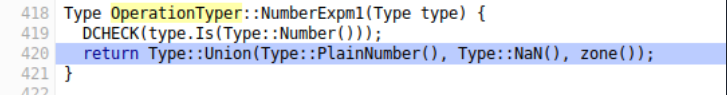
\includegraphics[width=\linewidth]{typer.png}
	\caption{The buggy return type declaration for Math.expm1() in operation-typer.cc}
  \label{fig:typer}
\end{figure}	
We will focus now on one of these bugs in particular. The TurboFan JIT compiler used by v8, the
JavaScript engine for the Chrome and Chromium web browsers, was exploited in 2018 using an edge case
with the function \texttt{Math.expm1()}, which computes $e^x -1$ for argument $x$.  Specifically, if
we evaluate \texttt{Math.expm1(-0)}, this should produce the value -0.  However, the TurboFan JIT
lists the return types for this function as a union of the \texttt{PlainNumber} type and NaN. This
union includes all values of a 64-bit floating point number, except -0. V8 defines this behavior
using a special table in typer.cc and operation-typer.cc. The code from the latter is shown in
Figure \ref{fig:typer}. The JIT uses this fine-grained type information to peform variable range
analysis that is used in array bounds check eliminations. For example, if TurboFan realizes a
boolean variable is used to index an array of length $\geq$ 2, then the native compiled code can
forgo ensuring the array index is in range, saving time. As we will see in the following section,
the mismatch between the expected and actual ouput range of \texttt{Math.expm1()} can have
catastrophic effects.

\section{Exploitation Techniques}
In this section we will walk through the process of exploiting the bug, all the way up to arbitrary
code execution. In our instance, we choose to spawn a shell.

\subsection{Triggering the Bug}

\begin{figure}
	\centering
	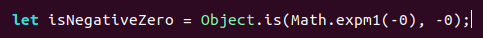
\includegraphics[width=300pt]{example1.png}
	\caption{Code which determines whether Math.expm1() returns 0 or -0}
  \label{fig:example1}
\end{figure}

The goal of the first stage of our exploit is to utilize the buggy fine-grained return type of
\texttt{Math.expm1()} to eliminate a bounds check which is in fact not safe, and allow us to access
memory outside the bounds of the array. The first step involves creating a variable which depends on
the result of our buggy function call. In other words, we need a way to distinguish between the
values 0 and -0. The only function useful to us in this case is \texttt{Object.is()}. In the code
segment shown in Figure \ref{fig:example1}, the variable \texttt{isNegativeZero} will be 1 if
\texttt{Math.expm1()} returns -0, and 0 otherwise. Running this line of code before it becomes 'hot'
and JIT optimzed will always store 1 into \texttt{isNegativeZero}, because the code is interpreted
directly and the native backing function for \texttt{Math.expm1()} returns -0. 

\begin{figure}
	\centering
	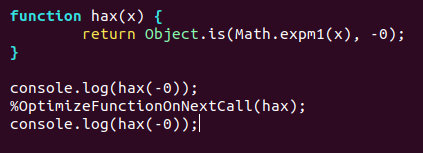
\includegraphics[width=300pt]{example2.png}
	\caption{The first call to hax() correctly prints 'true', but the second prints 'false' because the buggy JIT optimization folds the entire Object.is call to 'false'.}
  \label{fig:example2}
\end{figure}

This becomes interesting when we run the code after it has been JIT-optimized. Consider the code in
Figure \ref{fig:example2}. This code calls the function \texttt{hax} once without optimization, and
once with optimization. The \texttt{\%OptimizeFucntionOnNextCall} annotation is a macro which can be
invoked using the \texttt{--allow-natives-syntax} flag on the command line. These annotations are
only used for debugging, and in a real exploit this macro would be replaced with calling the
function a set number of times in a loop to achieve the level of optimization we want (Note that for
this to work, we have to start by passing in a number value, and then repeatedly pass in strings in
order to force the JIT to optimize based on a number argument, but then repeatedly bail out until we
reach the call in which we want to trigger the exploit, in order to force optimization to occur just
before the exploit call). Running this code prints \texttt{true} for the first call and
\texttt{false} for the second. Why? The first time the code runs, it is interpreted directly, and
the engine correctly evaluates -0 equal to -0. Before the second call, the JIT (incorrectly)
optimizes the function to native code, and in its analysis it incorrectly assumes
\texttt{Math.expm1()} can never return -0, since its return type is (erroneously) listed as a union
of \texttt{PlainNumber} and \texttt{NaN}. Therefore TurboFan assumes the \texttt{Object.is} call
always evaluates to \texttt{false}, and uses \textit{Folding} to reduce the variable
\texttt{isNegativeZero} to the constant \texttt{false}, thus breaking the semantics of the
\texttt{Math.expm1()} function.

\subsection{Triggering an Out-of-Bounds Array Access}
\begin{figure}
	\centering
	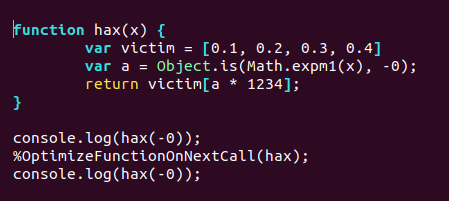
\includegraphics[width=300pt]{example3.png}
	\caption{First attempt at an out of bounds array access. This fails because the Object.is
	call folds to false, which prevents the out of bounds index.}
  \label{fig:example3}
\end{figure}
Now that we've triggered the bug, how can we turn it into a memory leak? The idea is to exploit the
bug to cause the JIT to remove an array bounds check in the optimized code, allowing us to read out
of bounds. Consider the code in Figure \ref{fig:example3}. The first time \texttt{hax} is called,
the function is interpreted directly and the engine realizes the variable \texttt{a} will be
\texttt{true}, meaning the index to \texttt{victim} will be out of bounds, and we will print
undefined. The second time, the function is optimized, and our goal is to cause the array bounds
check to be eliminated, while the variable \texttt{a} still evaluates to true. Although the bounds
check does in fact get removed, the \texttt{Object.is} call is still folded to \texttt{false}, so we
print 0.1, the first value in \texttt{victim} instead.

\begin{figure}
	\centering
	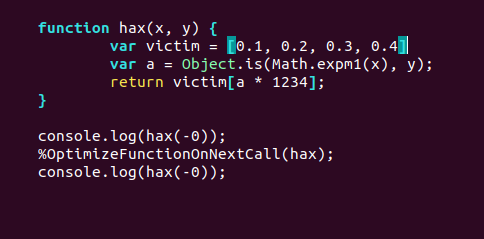
\includegraphics[width=300pt]{example5.png}
	\caption{Second attempt at an out of bounds array access. The Object.is call is no longer
	folded, but the variable \texttt{y} could be out of  the Object.is call folds to false,
	but this still fails because the bounds check is not removed.}
  \label{fig:example5}
\end{figure}

\subsubsection{Folding Prevention}
We can attempt to remove the folding by introducing indirection into the arguments to the
\texttt{Object.is} call. In the code in Figure \ref{fig:example5}, we replace the hard-coded value
-0 as the second argument with a function parameter \texttt{y}. If we run this, we get undefined for
the first call, and undefined for the second. The reason is that we successfully prevented the
folding, but the bounds check is no longer removed, because the JIT wants to account for alternate
values of \texttt{y} which are legitamately in the range of \texttt{Math.expm1}. We need some
mechanism of guaranteeing the value of \texttt{y} which will not fold the \texttt{Object.is} call.

\begin{figure}
	\centering
	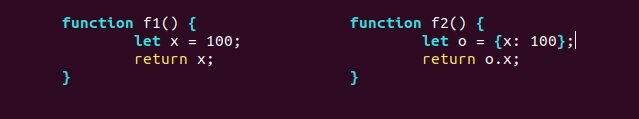
\includegraphics[width=400pt]{example4.png}
	\caption{Example of escape analysis.}
  \label{fig:example4}
\end{figure}

\subsubsection{Escape Analysis Manipulation}
The technique useful for this type of manipulation is escape analysis
manipulation. Consider the two code segments in Figure \ref{fig:example4}.
These two functions \texttt{f1} and \texttt{f2} have the same effect. In
\texttt{f1}, the object \texttt{o} is not necessary. TurboFan accordingly
optimizes objects like this out if their context does not escape the function.
If the object \texttt{o} were passed to an external function within
\texttt{f1}, the object would not be optimized. Escape analysis has some
useful side effects we can leverage. 
\begin{figure}
	\centering
	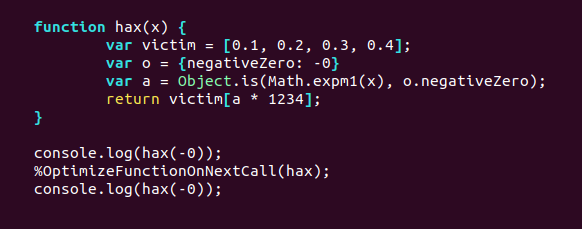
\includegraphics[width=300pt]{example6.png}
	\caption{Successful out of bounds memory access, using escape analsyis manipulation. The
	Object.is call is no longer folded, and the bounds check is eliminated.}
  \label{fig:example6}
\end{figure}
For example, consider the code in Figure \ref{fig:example6}.
The variable \texttt{o.negativeZero} is always the constant -0, but the indirection prevents
folding, while still allowing the range analysis to remove the bounds check under most
circumstances. We will point out that this range analysis elimination is particularly inconsistent,
and requirements may vary between versions, where subtle changes like even the length of the 
\texttt{victim} array can make a difference. In the CTF contest where this bug was discovered, the
modified version of v8 used for the event seemed to be much more consistent in removing the bounds
check than actual release versions. Nevertheless, it is possible, and if the bounds check succeeds,
we will read from \texttt{victim[1 * 1234] = victim[1234]}, which will print a garbage value from
memory. Of course we can change the value from 1234 to read other memory on the heap after the end
of the array.

\subsection{Obtaining Stable Out-of-Bounds Read and Write}
\begin{figure}
	\centering
	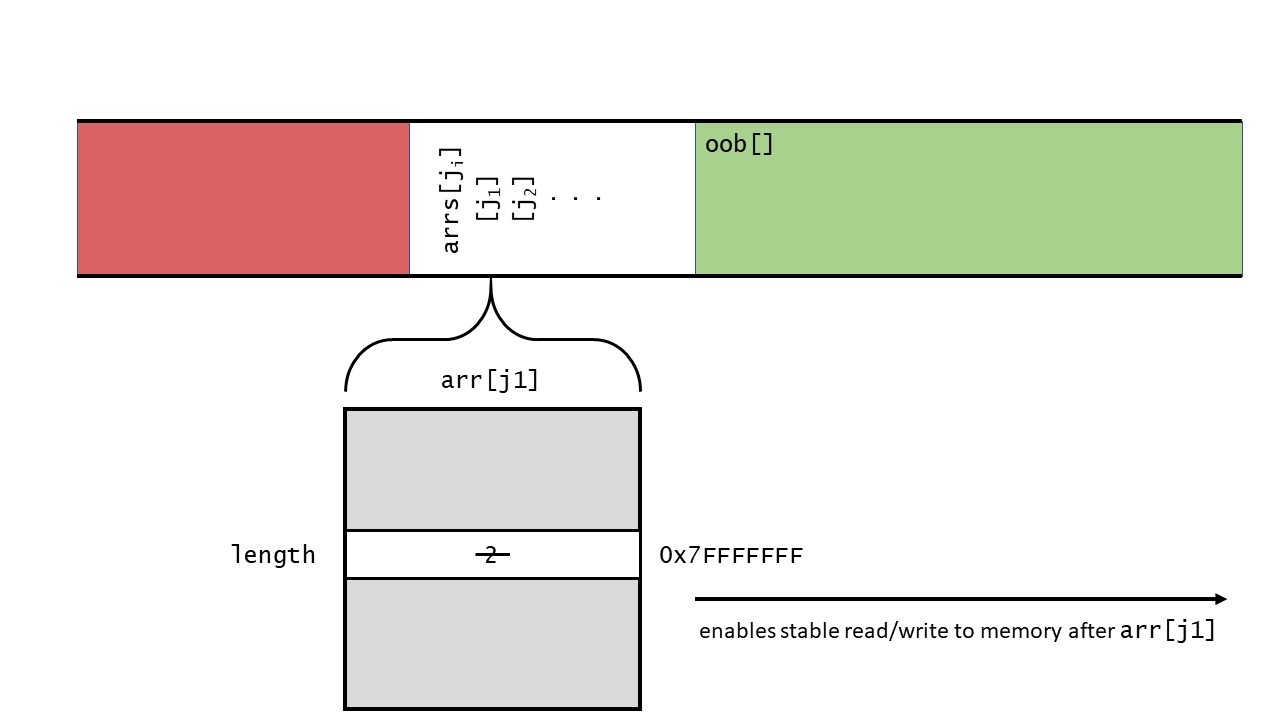
\includegraphics[width=\linewidth]{oob.jpg}
	\caption{Successful out of bounds memory access, using escape analsyis manipulation. The
	Object.is call is no longer folded, and the bounds check is eliminated.}
  \label{fig:oob}
\end{figure}

The \texttt{Math.expm1()} exploit allows us to read and write to memory out of bounds, but
triggering the bug for every out of bounds access necessary for the exploit is not optimal. We need
a more reliable out of bounds access. To do this, we spray arrays on the heap, each initially of
size 2, and use our unstable out of bounds read and write privilege to hopefully find metadata for
one of the arrays on the heap, and overwrite the length parameter in the metadata with
\texttt{0x7fffffff}, which corrupts the array to have much larger length than the memory allocated
to it. Then we loop through all of the sprayed arrays and detect if any of them have length larger
than 2. If we find such an array, it was the one we corrupted, and we can use it to reliably access
out of bounds and corrupt other objects. Figure \ref{fig:oob} shows a visual representation of the 
memory exploit for obtaining an unbounded array.

\subsection{Developing Exploitation Primitives}
In order to achieve code execution using our exploit, it is easiest to develop exploitation
primitives. In our exploit, we develop three: the \texttt{addrof()} primitive, which takes an object
and returns the memory address which stores the object's metadata, the \texttt{read()} primitive,
which returns a numerical value read from a given memory address, and the \texttt{write()}
primitive, which writes a given value to a given memory address. 

\subsubsection{Implementing \texttt{addrof()}}
\begin{figure}
	\centering
	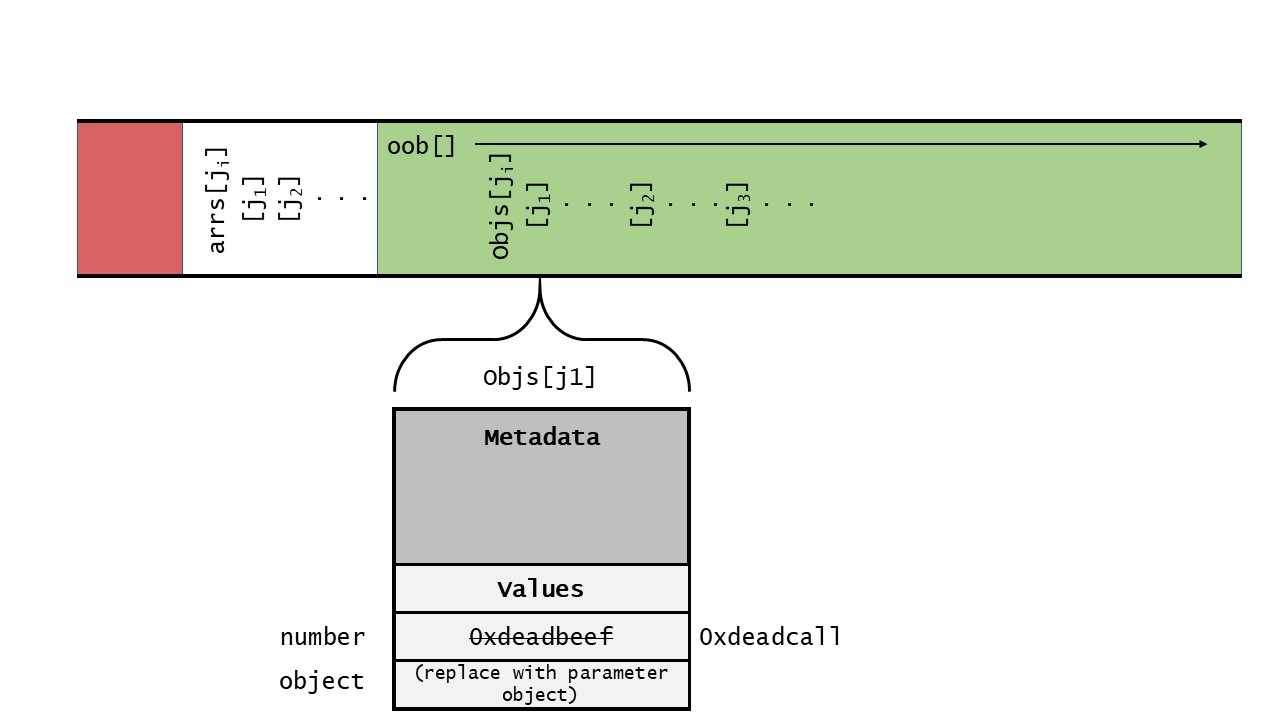
\includegraphics[width=\linewidth]{addrof.jpg}
	\caption{Successful out of bounds memory access, using escape analsyis manipulation. The
	Object.is call is no longer folded, and the bounds check is eliminated.}
  \label{fig:addrof}
\end{figure}
In order to obtain an object's memory address, we can utilize the way v8 (and most JavaScript
engines) store objects into variables. Instead of allocating JavaScript objects inline where the
variable is allocated, the variable data instead stores a pointer to the object's metadata in place
of where the value would be stored if the variable were a number. So we need a place to write an
object which we can detect the memory location of. We achieve this by spraying objects onto the heap
with two data elements: a hard-coded number field to server as a marker (we use the value
\texttt{0x1eadbeef}, and an object field which is initialized to an empty placeholder object. After
we spray the objects, we search the heap using our corrupted array and search for our marker value.
If we find it, the memory most likely corresponds to one of the objects we sprayed. Similar to the
sprayed arrays in the previous section, we overwrite this memory address with an alternate marker
value, and search the sprayed objects for this value to find the corresponding object. Finally, to
achieve \texttt{addrof()}, we simply store the argument object in the object field of the spray
object we found (which writes the argument object's memory address in the sprayed object), and then
read from memory at the index of the marker we found plus 8 bytes. This has the effect of returning
the argument object's memory address as a number, thus completing the primitive.  Figure
\ref{fig:addrof} shows a visual representation of the memory exploit for obtaining the
\texttt{addrof()} primitive.

\subsubsection{Implementing \texttt{read()} and \texttt{write()}}
\begin{figure}
	\centering
	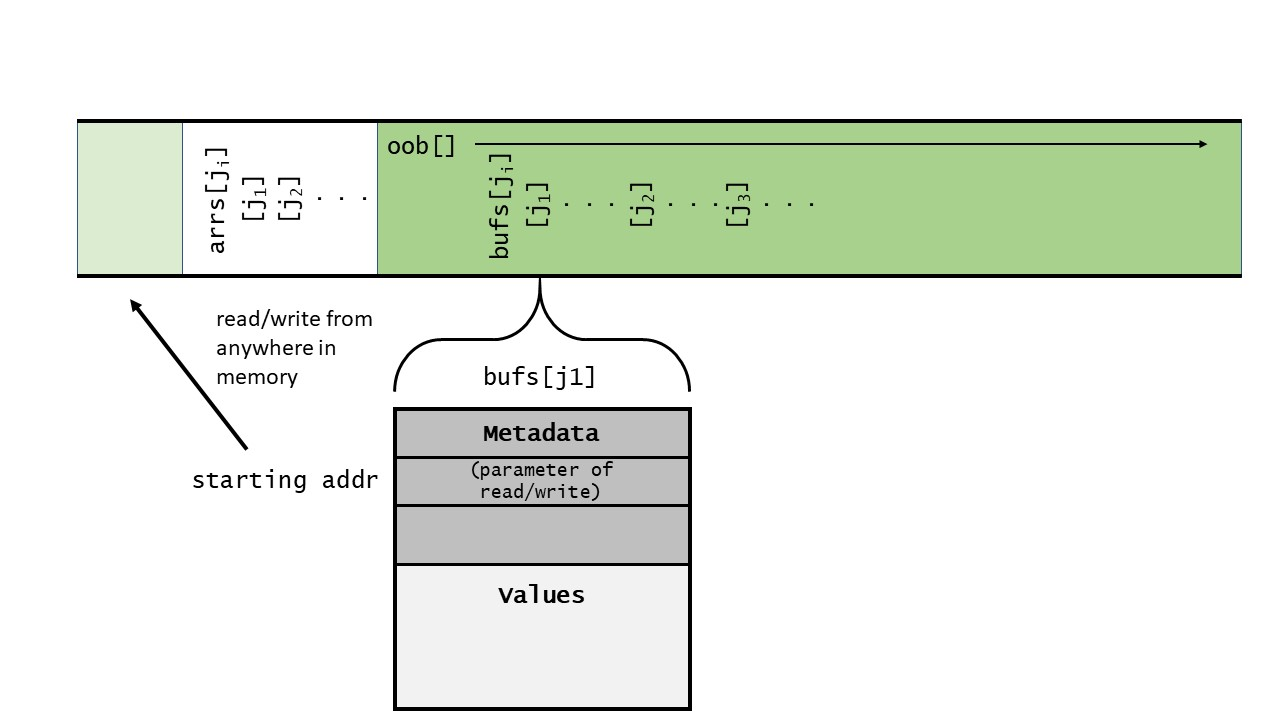
\includegraphics[width=\linewidth]{readmem.jpg}
	\caption{Successful out of bounds memory access, using escape analsyis manipulation. The
	Object.is call is no longer folded, and the bounds check is eliminated.}
  \label{fig:readmem}
\end{figure}
For aritrary read/write, we utilize the same technique as with \texttt{addrof()}, except we spray
\texttt{ArrayBuffer} objects, and pinpoints the memory location of the metadata using our out of
bounds access and a hard-coded paramter to the object we pass in. After we discover the memory
location of an ArrayBuffer, we mark it with a specific size to make it findable, and loop through
our list of sprayed buffers to find the object matching the memory location, we can overwrite the
start\_address pointer in the buffer metadata to point to the address of our choice, construct an
array using the array buffer, and read or write to the array at index 0, which points to our choice
memory address because of the metadata corruption. Thus we can now read and write to any memory
address we want. Figure \ref{fig:readmem} shows a visual representation of the memory exploit for
obtaining arbitrary read and write.

\subsection{Executing a Shell}
In order to spawn a shell, we utilize the fact that in v8, WebAssembly (WASM) memory pages are mapped
with read, write, and exceute permissions. We allocate a WASM page with placeholder code, leak its
location with \texttt{addrof()}, and overwrite the memory page with shellcode using our
\texttt{write()} primitive. Finally, we call the overwritten WASM segment as a function, and this
has the effect of executing our shellcode and spawns a shell, thus completing the exploit.


\begin{figure}
	\centering
	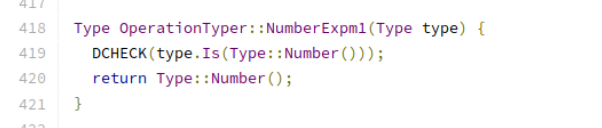
\includegraphics[width=300pt]{patch.png}
	\caption{The patched return type definition of \texttt{Math.expm1} in operation-typer.cc.}
  \label{fig:patch}
\end{figure}
\section{Patch and Resolution}
On September 5, 2018, v8 commit 56f7dda6 fixed the bug in operation-typer.cc, and later on October 15, commit 59c9c46b fixed the bug in typer.cc. Figure \ref{fig:patch} shows the segment of operation-typer.cc from Figure \ref{fig:typer} after the patch. Following this patch, the fine-grained return type of \texttt{Math.expm1} is redefined to \texttt{Number}, which includes -0, which prevents the JIT compiler from making any optimizations that could lead to out of bounds accesses as a result of passing in -0 to \texttt{Math.expm1()}.

\section{Acknowledgements} 
We would like to thank Andrea Biondo, who wrote some very nice analysis of this bug and how it was exploitable, at https://abiondo.me/2019/01/02/exploiting-math-expm1-v8/.

\begin{thebibliography}{}
	\bibitem{Grob}
		Groß, S. (2018).
	\bibitem{Biondo}
		Biondo, A. (2019, January 2). Exploiting the Math.expm1 typing bug in V8. Retrieved from https://abiondo.me/2019/01/02/exploiting-math-expm1-v8/.
	\bibitem{Bosamiya}
		Bosamiya, J. (2019, January 2). Exploiting Chrome V8: Krautflare (35C3 CTF 2018) . Retrieved from https://www.jaybosamiya.com/blog/2019/01/02/krautflare/.
	\bibitem{Issue}
		Issue 1710: Chrome: V8: incorrect type information on Math.expm1. (n.d.). Retrieved from https://bugs.chromium.org/p/project-zero/issues/detail?id=1710.
	\bibitem{Klees}
		Klees, G., Ruef, A., Cooper, B., Wei, S., \& Hicks, M. (2018). Evaluating Fuzz Testing. Proceedings of the 2018 ACM SIGSAC Conference on Computer and Communications Security - CCS 18. doi: 10.1145/3243734.3243804
	\bibitem{Saelo1}
		Saelo. (2016, October 27). Attacking JavaScript Engines: A case study of JavaScriptCore and CVE-2016-4622. Retrieved from http://phrack.org/papers/attacking\_javascript\_engines.html.
	\bibitem{Saelo2}
		Saelo. (2019, May 7). Exploiting Logic Bugs in JavaScript JIT Engines. Retrieved from http://www.phrack.org/papers/jit\_exploitation.html.
\end{thebibliography}

\end{document}

